% 2007 年重庆卷理科第 19 题：直三棱柱 ABC-A1B1C1，AA1=2，AB=1，∠ABC=90°；
%   D 在 BB1 上且 BD=(4/5)BB1，E 在 A1D 上且 B1E⊥A1D，四棱锥 C-ABDA1 与棱柱体积比 3:5。
% 来源 PDF：gaokaomath-src/普通高考/2007/2007重庆理.pdf
% SHA-256：83bfde9cfb8071229219565245c08cf4481943489659cb0f050919c380c65c3e
% 原页：2007重庆理.pdf 第 1 页（A3 三栏）第 3 栏，书页码 355。
% 重绘依据：按原页 A1、C1、B1、E、D、A、B、C 的相对位置与虚实线重绘；
%   E 取 A1D 上参数 25/29 处（即 B1 到 A1D 的垂足），使 A1—E—D 共线。
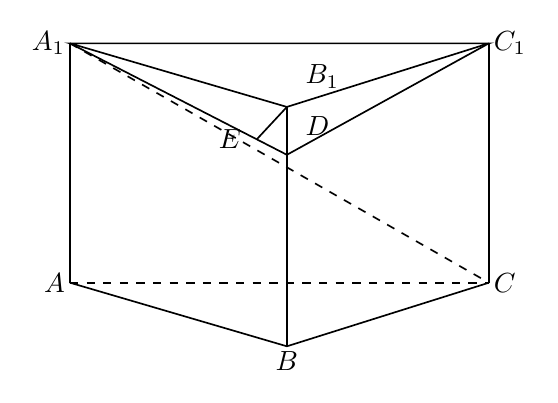
\begin{tikzpicture}[scale=0.95, semithick,
  every node/.style={inner sep=1.5pt}]

  \coordinate (A)  at (0.0,1.20);
  \coordinate (B)  at (2.90,0.35);
  \coordinate (C)  at (5.60,1.20);
  \coordinate (A1) at (0.0,4.40);
  \coordinate (B1) at (2.90,3.55);
  \coordinate (C1) at (5.60,4.40);
  \coordinate (D)  at (2.90,2.91);
  \coordinate (E)  at (2.50,3.12);

  % 底面
  \draw (A) -- (B) -- (C);
  \draw[dashed] (A) -- (C);
  % 侧棱
  \draw (A) -- (A1);
  \draw (B) -- (B1);
  \draw (C) -- (C1);
  % 上底面
  \draw (A1) -- (B1) -- (C1) -- cycle;

  % 题设连线
  \draw (A1) -- (D);
  \draw (B1) -- (E);
  \draw (D) -- (C1);
  \draw[dashed] (A1) -- (C);

  \node[left] at (A) {$A$};
  \node[below] at (B) {$B$};
  \node[right] at (C) {$C$};
  \node[left] at (A1) {$A_1$};
  \node[above right=5pt] at (B1) {$B_1$};
  \node[right] at (C1) {$C_1$};
  \node[above right=5pt] at (D) {$D$};
  \node[left=4pt] at (E) {$E$};
\end{tikzpicture}
